% Options for packages loaded elsewhere
\PassOptionsToPackage{unicode}{hyperref}
\PassOptionsToPackage{hyphens}{url}
%
\documentclass[
]{book}
\usepackage{lmodern}
\usepackage{amsmath}
\usepackage{ifxetex,ifluatex}
\ifnum 0\ifxetex 1\fi\ifluatex 1\fi=0 % if pdftex
  \usepackage[T1]{fontenc}
  \usepackage[utf8]{inputenc}
  \usepackage{textcomp} % provide euro and other symbols
  \usepackage{amssymb}
\else % if luatex or xetex
  \usepackage{unicode-math}
  \defaultfontfeatures{Scale=MatchLowercase}
  \defaultfontfeatures[\rmfamily]{Ligatures=TeX,Scale=1}
\fi
% Use upquote if available, for straight quotes in verbatim environments
\IfFileExists{upquote.sty}{\usepackage{upquote}}{}
\IfFileExists{microtype.sty}{% use microtype if available
  \usepackage[]{microtype}
  \UseMicrotypeSet[protrusion]{basicmath} % disable protrusion for tt fonts
}{}
\makeatletter
\@ifundefined{KOMAClassName}{% if non-KOMA class
  \IfFileExists{parskip.sty}{%
    \usepackage{parskip}
  }{% else
    \setlength{\parindent}{0pt}
    \setlength{\parskip}{6pt plus 2pt minus 1pt}}
}{% if KOMA class
  \KOMAoptions{parskip=half}}
\makeatother
\usepackage{xcolor}
\IfFileExists{xurl.sty}{\usepackage{xurl}}{} % add URL line breaks if available
\IfFileExists{bookmark.sty}{\usepackage{bookmark}}{\usepackage{hyperref}}
\hypersetup{
  pdftitle={Master's Thesis Research},
  pdfauthor={Ronan Hart},
  hidelinks,
  pdfcreator={LaTeX via pandoc}}
\urlstyle{same} % disable monospaced font for URLs
\usepackage{color}
\usepackage{fancyvrb}
\newcommand{\VerbBar}{|}
\newcommand{\VERB}{\Verb[commandchars=\\\{\}]}
\DefineVerbatimEnvironment{Highlighting}{Verbatim}{commandchars=\\\{\}}
% Add ',fontsize=\small' for more characters per line
\usepackage{framed}
\definecolor{shadecolor}{RGB}{248,248,248}
\newenvironment{Shaded}{\begin{snugshade}}{\end{snugshade}}
\newcommand{\AlertTok}[1]{\textcolor[rgb]{0.94,0.16,0.16}{#1}}
\newcommand{\AnnotationTok}[1]{\textcolor[rgb]{0.56,0.35,0.01}{\textbf{\textit{#1}}}}
\newcommand{\AttributeTok}[1]{\textcolor[rgb]{0.77,0.63,0.00}{#1}}
\newcommand{\BaseNTok}[1]{\textcolor[rgb]{0.00,0.00,0.81}{#1}}
\newcommand{\BuiltInTok}[1]{#1}
\newcommand{\CharTok}[1]{\textcolor[rgb]{0.31,0.60,0.02}{#1}}
\newcommand{\CommentTok}[1]{\textcolor[rgb]{0.56,0.35,0.01}{\textit{#1}}}
\newcommand{\CommentVarTok}[1]{\textcolor[rgb]{0.56,0.35,0.01}{\textbf{\textit{#1}}}}
\newcommand{\ConstantTok}[1]{\textcolor[rgb]{0.00,0.00,0.00}{#1}}
\newcommand{\ControlFlowTok}[1]{\textcolor[rgb]{0.13,0.29,0.53}{\textbf{#1}}}
\newcommand{\DataTypeTok}[1]{\textcolor[rgb]{0.13,0.29,0.53}{#1}}
\newcommand{\DecValTok}[1]{\textcolor[rgb]{0.00,0.00,0.81}{#1}}
\newcommand{\DocumentationTok}[1]{\textcolor[rgb]{0.56,0.35,0.01}{\textbf{\textit{#1}}}}
\newcommand{\ErrorTok}[1]{\textcolor[rgb]{0.64,0.00,0.00}{\textbf{#1}}}
\newcommand{\ExtensionTok}[1]{#1}
\newcommand{\FloatTok}[1]{\textcolor[rgb]{0.00,0.00,0.81}{#1}}
\newcommand{\FunctionTok}[1]{\textcolor[rgb]{0.00,0.00,0.00}{#1}}
\newcommand{\ImportTok}[1]{#1}
\newcommand{\InformationTok}[1]{\textcolor[rgb]{0.56,0.35,0.01}{\textbf{\textit{#1}}}}
\newcommand{\KeywordTok}[1]{\textcolor[rgb]{0.13,0.29,0.53}{\textbf{#1}}}
\newcommand{\NormalTok}[1]{#1}
\newcommand{\OperatorTok}[1]{\textcolor[rgb]{0.81,0.36,0.00}{\textbf{#1}}}
\newcommand{\OtherTok}[1]{\textcolor[rgb]{0.56,0.35,0.01}{#1}}
\newcommand{\PreprocessorTok}[1]{\textcolor[rgb]{0.56,0.35,0.01}{\textit{#1}}}
\newcommand{\RegionMarkerTok}[1]{#1}
\newcommand{\SpecialCharTok}[1]{\textcolor[rgb]{0.00,0.00,0.00}{#1}}
\newcommand{\SpecialStringTok}[1]{\textcolor[rgb]{0.31,0.60,0.02}{#1}}
\newcommand{\StringTok}[1]{\textcolor[rgb]{0.31,0.60,0.02}{#1}}
\newcommand{\VariableTok}[1]{\textcolor[rgb]{0.00,0.00,0.00}{#1}}
\newcommand{\VerbatimStringTok}[1]{\textcolor[rgb]{0.31,0.60,0.02}{#1}}
\newcommand{\WarningTok}[1]{\textcolor[rgb]{0.56,0.35,0.01}{\textbf{\textit{#1}}}}
\usepackage{longtable,booktabs}
\usepackage{calc} % for calculating minipage widths
% Correct order of tables after \paragraph or \subparagraph
\usepackage{etoolbox}
\makeatletter
\patchcmd\longtable{\par}{\if@noskipsec\mbox{}\fi\par}{}{}
\makeatother
% Allow footnotes in longtable head/foot
\IfFileExists{footnotehyper.sty}{\usepackage{footnotehyper}}{\usepackage{footnote}}
\makesavenoteenv{longtable}
\usepackage{graphicx}
\makeatletter
\def\maxwidth{\ifdim\Gin@nat@width>\linewidth\linewidth\else\Gin@nat@width\fi}
\def\maxheight{\ifdim\Gin@nat@height>\textheight\textheight\else\Gin@nat@height\fi}
\makeatother
% Scale images if necessary, so that they will not overflow the page
% margins by default, and it is still possible to overwrite the defaults
% using explicit options in \includegraphics[width, height, ...]{}
\setkeys{Gin}{width=\maxwidth,height=\maxheight,keepaspectratio}
% Set default figure placement to htbp
\makeatletter
\def\fps@figure{htbp}
\makeatother
\setlength{\emergencystretch}{3em} % prevent overfull lines
\providecommand{\tightlist}{%
  \setlength{\itemsep}{0pt}\setlength{\parskip}{0pt}}
\setcounter{secnumdepth}{5}
\usepackage{booktabs}
\ifluatex
  \usepackage{selnolig}  % disable illegal ligatures
\fi
\usepackage[]{natbib}
\bibliographystyle{apalike}

\title{Master's Thesis Research}
\author{Ronan Hart}
\date{2021-03-04}

\begin{document}
\maketitle

{
\setcounter{tocdepth}{1}
\tableofcontents
}
\hypertarget{masters-thesis-project}{%
\chapter{Master's Thesis Project}\label{masters-thesis-project}}

Quantifying the Impacts of Anthropogenic Movement Barriers on Ungulate Space-Use Patterns and Functional Connectivity in Utah

\hypertarget{abstract}{%
\section{Abstract}\label{abstract}}

Movement is an essential function for large herbivores to acquire resources and to avoid predation risk. The successful execution, and thus the functional value, of movement is dependent on the connectivity of the landscape. Impediments to movement, such as anthropogenic barriers, can impact space-use behaviors and cause functional habitat loss and fragmentation. Disruptions to landscape connectivity can increase mortality, block gene flow, increase a population's vulnerability to extirpation, and compromise metapopulation persistence. Furthermore, because functional landscape connectivity is species- and context-dependent, it is necessary to be scrutinous and examine animal movement by multiple species and in a variety of spatial-temporal contexts to understand the full scope of barrier impacts on functional connectivity. To address this, our research will look at two ungulate species in Utah -- mule deer (Odocoileus hemionus) and pronghorn (Antilocapra americana) -- that share similar movement patterns and geographic space but require different ecological needs and reside in, and move through, different habitats. These two species provide a unique opportunity to compare their space-use shifts around barriers and therefore gain a holistic understanding of functional habitat loss in the many landscapes across Utah. I will use GPS-collar data provided by the Utah Division of Wildlife Resources (UDWR) to analyze individual movement with respect to roads, fences, landcover, vegetation, and snow depth using integrated step selection analysis (iSSA). I plan to provide a comprehensive picture of landscape connectivity in a variable landscape with multiple species. This will give wildlife managers with essential tools to mitigate current barrier effects and aid in predicting impacts from future barrier construction.

\hypertarget{questions}{%
\section{Questions}\label{questions}}

I seek to answer four main questions

\begin{enumerate}
\def\labelenumi{\arabic{enumi}.}
\tightlist
\item
  Do barriers impact pronghorn differently than they impact mule deer?
\item
  How do barrier impacts differ between seasons?
\item
  How do barrier impacts differ between individuals and populations exhibiting different movement patterns?
\item
  Do barrier impacts vary in different habitat types?
\end{enumerate}

\hypertarget{objectives}{%
\section{Objectives}\label{objectives}}

\begin{enumerate}
\def\labelenumi{\arabic{enumi}.}
\tightlist
\item
  Determine the probability of crossing a barrier. I will consider probability to be a function of species, barrier attributes traffic volume, number of lanes, fence type, and fence height), and the local environmental attributes (time of day, season, elevation, vegetation type and quality, and snow depth).
\item
  Quantify behavioral responses around roads and fences to estimate functional habitat loss due to proximity avoidance.
\item
  Develop maps showing habitat loss and fragmentation due to barrier impacts.
\item
  Develop maps of the relative probability of barrier crossing and avoidance given the environmental attributes of each point in the map.
\item
  Use these maps to determine where and when barriers cause the highest degradation, predict how future barrier construction could impact habitats, and predict how barrier modification could mitigate impacts.\\
\end{enumerate}

\hypertarget{db_structure}{%
\chapter{Database Structure}\label{db_structure}}

\hypertarget{database-structure}{%
\section{Database Structure}\label{database-structure}}

To best structure all of my data, I will be storing my datasets into a database. My data will be in 3 main categories:

\begin{itemize}
\tightlist
\item
  GPS data from collared pronghorn and mule deer
\item
  Barrier locations and attributes (roads, fences, railroads, etc.)
\item
  Environmental covariates

  \begin{itemize}
  \tightlist
  \item
    Elevation
  \item
    Landcover
  \item
    Vegetation type and phenology
  \item
    Snow depth
  \end{itemize}
\end{itemize}

\textbackslash begin\{figure\}

\{\centering 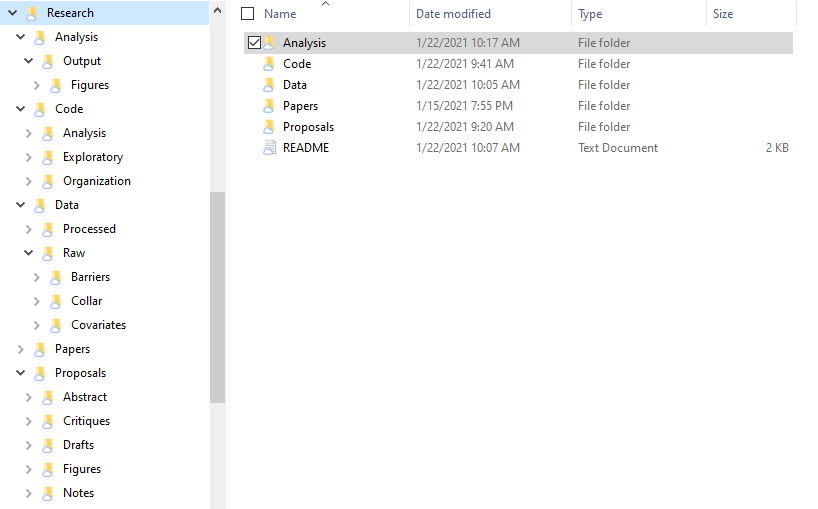
\includegraphics[width=0.7\linewidth]{../Database/Directory Structure}

\}

\caption{Directory Structure}

(\#fig:dir\_pic)
\textbackslash end\{figure\}

The above picture shows my directory structure for this project. This directory reflects an Activity-based organization, with all the code stored in one folder, all the data stored in one folder, etc.

\textbackslash begin\{figure\}

\{\centering 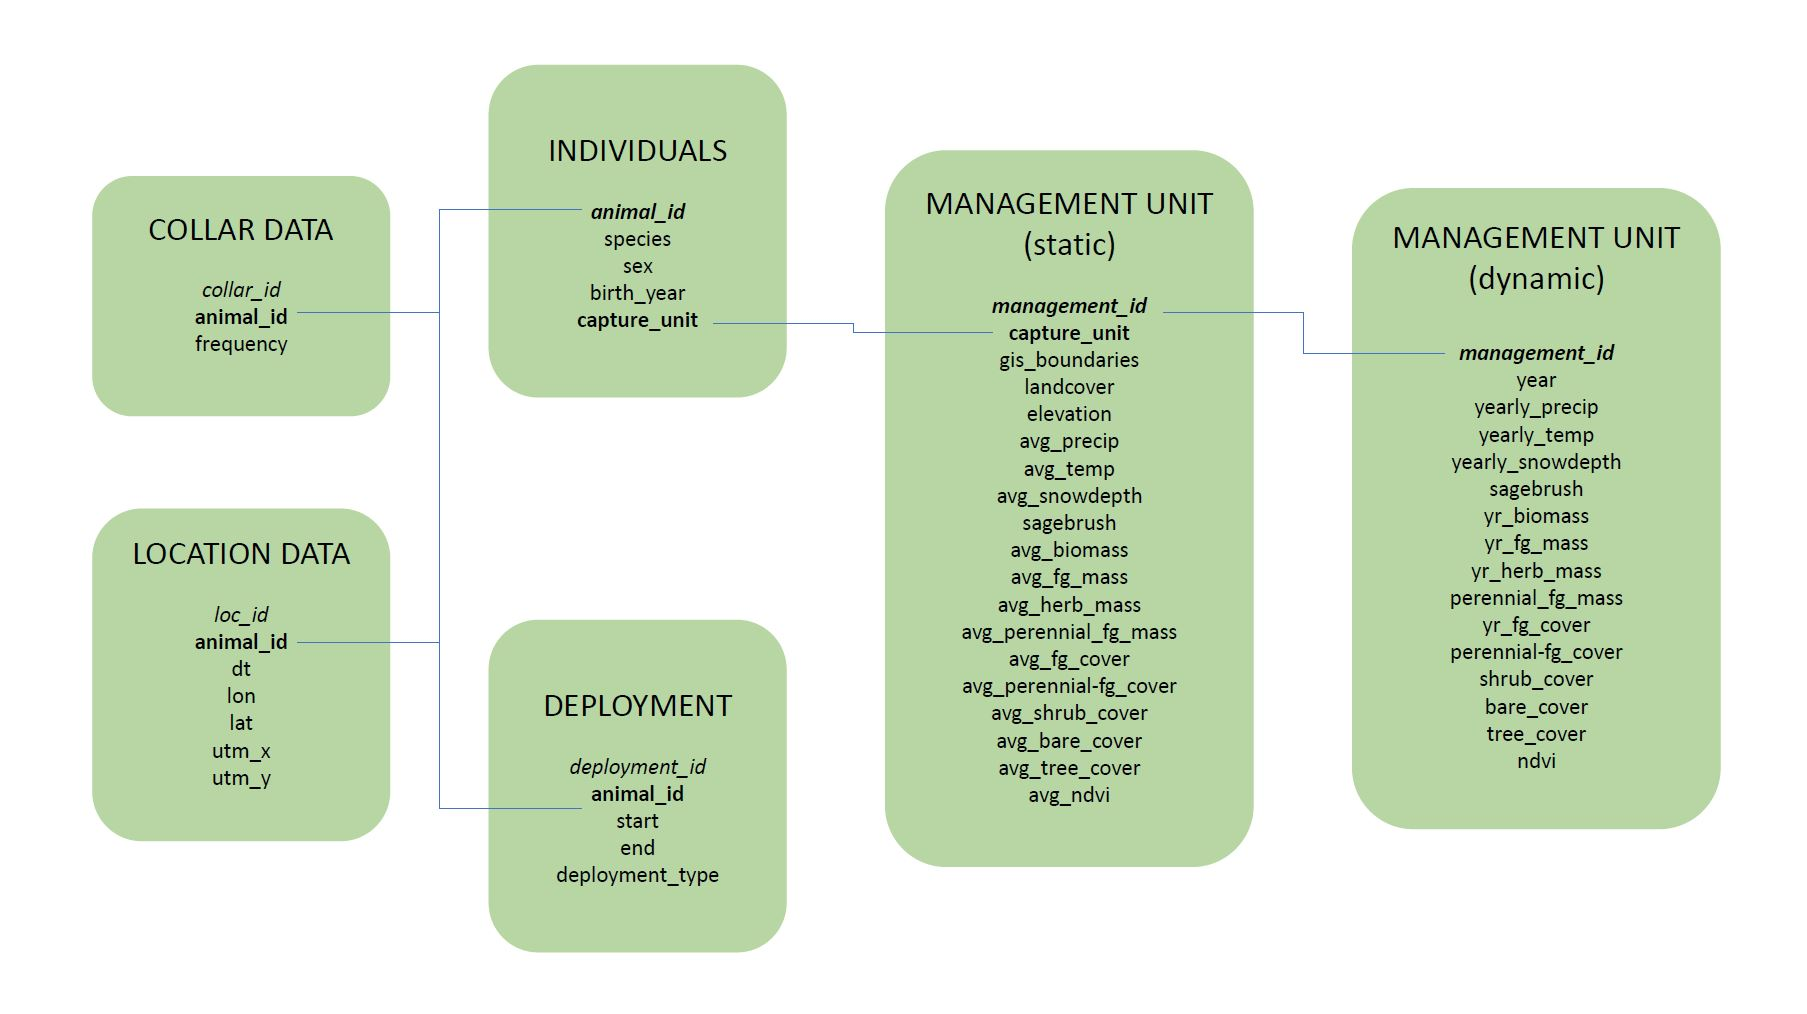
\includegraphics[width=0.9\linewidth]{../Database/Database_Structure}

\}

\caption{Database Structure}

(\#fig:db\_pic)
\textbackslash end\{figure\}

The above picture shows my database structure. Most of this database is of the GPS data from collared animals. The majority of data of barriers and environmental covariates will be in the form of shapefiles or rasters, and so were not included in this database structure.

\hypertarget{forming-the-database}{%
\section{Forming the Database}\label{forming-the-database}}

Before I can begin working in RSQLite, I have to first format my raw data into a structure matching my planned structure above.

\textbackslash begin\{figure\}

\{\centering 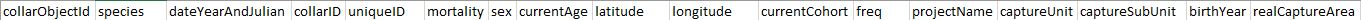
\includegraphics[width=1\linewidth]{../Database/colnames}

\}

\caption{Column Names of Raw Data}

(\#fig:raw\_dat\_pic)
\textbackslash end\{figure\}

To format my dataframes, I will be working with the packages \texttt{dplyr} -- which allows me to manipulate dataframes -- and \texttt{lubridate} -- which allows me to work with date and time formats.

\begin{Shaded}
\begin{Highlighting}[]
\CommentTok{\# Install Packages{-}{-}{-}{-}}
\FunctionTok{install.packages}\NormalTok{(}\StringTok{"dplyr"}\NormalTok{)}
\FunctionTok{install.packages}\NormalTok{(}\StringTok{"lubridate"}\NormalTok{)}
\end{Highlighting}
\end{Shaded}

\begin{Shaded}
\begin{Highlighting}[]
\CommentTok{\# Load Packages {-}{-}{-}{-}}
\FunctionTok{library}\NormalTok{(dplyr)}
\FunctionTok{library}\NormalTok{(lubridate)}
\end{Highlighting}
\end{Shaded}

\hypertarget{base-format}{%
\subsection{Base Format}\label{base-format}}

\emph{Note: I want to apologize to seasoned R coders that I come from a python background and I refuse to use \texttt{\textless{}-} as an assignment operator (too many keystrokes!). Instead, I use \texttt{=}.}

\begin{Shaded}
\begin{Highlighting}[]
\CommentTok{\# Load Data {-}{-}{-}{-}}
\NormalTok{df }\OtherTok{=} \FunctionTok{read.csv}\NormalTok{(}\StringTok{"../Data/Raw/GPS/full\_data.csv"}\NormalTok{)}
\end{Highlighting}
\end{Shaded}

\emph{Note: For the purposes of this demonstration, I have subset my data and randomized certain elements}

Let's take a look at the data

\begin{Shaded}
\begin{Highlighting}[]
\FunctionTok{head}\NormalTok{(df)}
\end{Highlighting}
\end{Shaded}

\begin{verbatim}
##   X collarObjectId   species   dateYearAndJulian collarID  uniqueID mortality
## 1 1         171976 mule deer 2014-12-08 02:00:00    34895 MD13F0035     false
## 2 2         171977 mule deer 2014-12-08 14:00:00    34895 MD13F0035     false
## 3 3         171978 mule deer 2014-12-09 15:00:00    34895 MD13F0035     false
## 4 4         171979 mule deer 2014-12-10 04:00:00    34895 MD13F0035     false
## 5 5         171980 mule deer 2014-12-10 16:00:00    34895 MD13F0035     false
## 6 6         170147 mule deer 2014-12-13 00:00:00    30261 MD14F0046     false
##   sex currentAge latitude longitude currentCohort     freq projectName
## 1   F        2.5 40.61487 -109.2107         adult 150.7638        <NA>
## 2   F        2.5 40.60612 -109.1469         adult 150.6706        <NA>
## 3   F        2.5 41.05850 -109.1184         adult 151.9882        <NA>
## 4   F        2.5 41.08347 -109.0206         adult 152.9788        <NA>
## 5   F        2.5 41.18861 -108.8705         adult 150.2661        <NA>
## 6   F        5.0 41.16767 -111.6087         adult 155.0224        <NA>
##         captureUnit captureSubUnit birthYear realCaptureArea
## 1       South Slope    Diamond Mtn      2013         Diamond
## 2       South Slope    Diamond Mtn      2013         Diamond
## 3       South Slope    Diamond Mtn      2013         Diamond
## 4       South Slope    Diamond Mtn      2013         Diamond
## 5       South Slope    Diamond Mtn      2013         Diamond
## 6 Oquirrh-Stansbury           <NA>      2010     Pine Canyon
\end{verbatim}

First I need to format my full data into a base format:

\begin{itemize}
\tightlist
\item
  change datetime column to class \texttt{POSIXct}
\end{itemize}

\begin{Shaded}
\begin{Highlighting}[]
\NormalTok{df }\OtherTok{=}\NormalTok{ df }\SpecialCharTok{\%\textgreater{}\%}
  \CommentTok{\# create a new column called "dt" (meaning "datetime")}
  \FunctionTok{mutate}\NormalTok{(}\AttributeTok{dt =} \FunctionTok{ymd\_hms}\NormalTok{(dateYearAndJulian))}
\end{Highlighting}
\end{Shaded}

\begin{itemize}
\tightlist
\item
  change mortality to \texttt{logical} class
\end{itemize}

\begin{Shaded}
\begin{Highlighting}[]
\NormalTok{df }\OtherTok{=}\NormalTok{ df }\SpecialCharTok{\%\textgreater{}\%}
  \FunctionTok{mutate}\NormalTok{(}\AttributeTok{mort =} \FunctionTok{as.logical}\NormalTok{(mortality))}
\end{Highlighting}
\end{Shaded}

\begin{itemize}
\tightlist
\item
  add a record ID for each record
\end{itemize}

\begin{Shaded}
\begin{Highlighting}[]
\NormalTok{df }\OtherTok{=}\NormalTok{ df }\SpecialCharTok{\%\textgreater{}\%}
  \FunctionTok{mutate}\NormalTok{(}\AttributeTok{rec\_id =} \FunctionTok{seq}\NormalTok{(}\DecValTok{1}\SpecialCharTok{:}\FunctionTok{nrow}\NormalTok{(df)))}
\end{Highlighting}
\end{Shaded}

\begin{itemize}
\tightlist
\item
  rename columns to a preferred format
\item
  select only the needed columns.
\end{itemize}

\begin{Shaded}
\begin{Highlighting}[]
\NormalTok{df }\OtherTok{=}\NormalTok{ df }\SpecialCharTok{\%\textgreater{}\%}
  \FunctionTok{select}\NormalTok{(rec\_id, }
         \AttributeTok{animal\_id =}\NormalTok{ uniqueID,}
\NormalTok{         species,}
\NormalTok{         sex,}
\NormalTok{         dt,}
         \CommentTok{\# added y and x so I can remember which one is which}
         \AttributeTok{lat\_y =}\NormalTok{ latitude,}
         \AttributeTok{lon\_x =}\NormalTok{ longitude,}
         \AttributeTok{cohort =}\NormalTok{ currentCohort,}
         \AttributeTok{birth\_year =}\NormalTok{ birthYear,}
         \AttributeTok{mortality =}\NormalTok{ mort,}
         \AttributeTok{capture\_unit =}\NormalTok{ captureUnit,}
         \AttributeTok{collar\_id =}\NormalTok{ collarID,}
         \AttributeTok{collar\_obj\_id =}\NormalTok{ collarObjectId,}
\NormalTok{         freq,}
         \AttributeTok{proj =}\NormalTok{ projectName)}
\end{Highlighting}
\end{Shaded}

Let's see what the data looks like now

\begin{Shaded}
\begin{Highlighting}[]
\FunctionTok{head}\NormalTok{(df)}
\end{Highlighting}
\end{Shaded}

\begin{verbatim}
##   rec_id animal_id   species sex                  dt    lat_y     lon_x cohort
## 1      1 MD13F0035 mule deer   F 2014-12-08 02:00:00 40.61487 -109.2107  adult
## 2      2 MD13F0035 mule deer   F 2014-12-08 14:00:00 40.60612 -109.1469  adult
## 3      3 MD13F0035 mule deer   F 2014-12-09 15:00:00 41.05850 -109.1184  adult
## 4      4 MD13F0035 mule deer   F 2014-12-10 04:00:00 41.08347 -109.0206  adult
## 5      5 MD13F0035 mule deer   F 2014-12-10 16:00:00 41.18861 -108.8705  adult
## 6      6 MD14F0046 mule deer   F 2014-12-13 00:00:00 41.16767 -111.6087  adult
##   birth_year mortality      capture_unit collar_id collar_obj_id     freq proj
## 1       2013     FALSE       South Slope     34895        171976 150.7638 <NA>
## 2       2013     FALSE       South Slope     34895        171977 150.6706 <NA>
## 3       2013     FALSE       South Slope     34895        171978 151.9882 <NA>
## 4       2013     FALSE       South Slope     34895        171979 152.9788 <NA>
## 5       2013     FALSE       South Slope     34895        171980 150.2661 <NA>
## 6       2010     FALSE Oquirrh-Stansbury     30261        170147 155.0224 <NA>
\end{verbatim}

Looks great!

\hypertarget{sort-into-different-datasets}{%
\subsection{Sort into Different Datasets}\label{sort-into-different-datasets}}

Now I can begin to sort into the different datasets for my final database structure

\hypertarget{individuals-dataset}{%
\subsubsection{Individuals Dataset}\label{individuals-dataset}}

\begin{Shaded}
\begin{Highlighting}[]
\NormalTok{indiv }\OtherTok{=}\NormalTok{ df }\SpecialCharTok{\%\textgreater{}\%}
  \FunctionTok{select}\NormalTok{(animal\_id, }\CommentTok{\# this will be the primary key and a foreign key}
\NormalTok{         species,}
\NormalTok{         sex,}
\NormalTok{         birth\_year,}
\NormalTok{         capture\_unit) }\SpecialCharTok{\%\textgreater{}\%}
  \FunctionTok{distinct}\NormalTok{()}

\FunctionTok{print}\NormalTok{(indiv)}
\end{Highlighting}
\end{Shaded}

\begin{verbatim}
##   animal_id   species sex birth_year      capture_unit
## 1 MD13F0035 mule deer   F       2013       South Slope
## 2 MD14F0046 mule deer   F       2010 Oquirrh-Stansbury
## 3 MD11F0041 mule deer   F       2009 Oquirrh-Stansbury
## 4 MD12U0015 mule deer   U       2014 Oquirrh-Stansbury
## 5 MD14M0027 mule deer   M       2011         Box Elder
\end{verbatim}

This table now shows our individual animals and their sex, species, birth year, and the management unit where they were captured.

Now we can save this table for later. I'll save it as a .rds file so that it keeps the format and datatypes and so it takes up less disk space.

\begin{Shaded}
\begin{Highlighting}[]
\FunctionTok{saveRDS}\NormalTok{(indiv, }\StringTok{"../Data/Processed/individual.rds"}\NormalTok{)}
\end{Highlighting}
\end{Shaded}

\hypertarget{collar-dataset}{%
\subsubsection{Collar Dataset}\label{collar-dataset}}

\begin{Shaded}
\begin{Highlighting}[]
\NormalTok{collar }\OtherTok{=}\NormalTok{ df }\SpecialCharTok{\%\textgreater{}\%}
  \FunctionTok{select}\NormalTok{(collar\_id, }\CommentTok{\# will be the primary key}
\NormalTok{         animal\_id) }\SpecialCharTok{\%\textgreater{}\%} \CommentTok{\# will be a foreign key}
  \FunctionTok{distinct}\NormalTok{() }\CommentTok{\# make sure all records are distinct}

\FunctionTok{print}\NormalTok{(collar)}
\end{Highlighting}
\end{Shaded}

\begin{verbatim}
##   collar_id animal_id
## 1     34895 MD13F0035
## 2     30261 MD14F0046
## 3     34265 MD11F0041
## 4     32680 MD12U0015
## 5     33655 MD14M0027
\end{verbatim}

Now we have a table showing our animals and their collar IDs. In this subset of data, these 5 individuals had the same collar the whole time. But in my real dataset, there are some animals that had more than one collar. So instead of \texttt{collar\_id} being stored with the ``individuals'' table, ``collar'' is its own table.

I'll also save this as a .rds file

\begin{Shaded}
\begin{Highlighting}[]
\FunctionTok{saveRDS}\NormalTok{(collar, }\StringTok{"../Data/Processed/collar.rds"}\NormalTok{)}
\end{Highlighting}
\end{Shaded}

\hypertarget{location-dataset}{%
\subsubsection{Location Dataset}\label{location-dataset}}

\begin{Shaded}
\begin{Highlighting}[]
\NormalTok{gps }\OtherTok{=}\NormalTok{  df }\SpecialCharTok{\%\textgreater{}\%}
  \CommentTok{\# create a new column loc\_id, a unique id for each location record}
  \FunctionTok{mutate}\NormalTok{(}\AttributeTok{loc\_id =} \FunctionTok{rep}\NormalTok{(}\DecValTok{1}\SpecialCharTok{:}\FunctionTok{nrow}\NormalTok{(df))) }\SpecialCharTok{\%\textgreater{}\%}
  \CommentTok{\# sort into new df only with columns related to location data}
  \FunctionTok{select}\NormalTok{(loc\_id, }\CommentTok{\# this will be the primary key}
\NormalTok{         animal\_id, }\CommentTok{\# this will be a foreign key}
\NormalTok{         dt,}
\NormalTok{         lat\_y,}
\NormalTok{         lon\_x)}

\FunctionTok{head}\NormalTok{(gps)}
\end{Highlighting}
\end{Shaded}

\begin{verbatim}
##   loc_id animal_id                  dt    lat_y     lon_x
## 1      1 MD13F0035 2014-12-08 02:00:00 40.61487 -109.2107
## 2      2 MD13F0035 2014-12-08 14:00:00 40.60612 -109.1469
## 3      3 MD13F0035 2014-12-09 15:00:00 41.05850 -109.1184
## 4      4 MD13F0035 2014-12-10 04:00:00 41.08347 -109.0206
## 5      5 MD13F0035 2014-12-10 16:00:00 41.18861 -108.8705
## 6      6 MD14F0046 2014-12-13 00:00:00 41.16767 -111.6087
\end{verbatim}

For the Location datset, I also need to add a column for UTM x and UTM y. My study area is in Utah, which is UTM Zone 12N. To convert to UTM, I need to use the package \texttt{sf}.

\begin{Shaded}
\begin{Highlighting}[]
\CommentTok{\# Install Packages {-}{-}{-}{-}}
\FunctionTok{install.packages}\NormalTok{(}\StringTok{"sf"}\NormalTok{)}
\end{Highlighting}
\end{Shaded}

\begin{Shaded}
\begin{Highlighting}[]
\CommentTok{\# Load Packages}
\FunctionTok{library}\NormalTok{(sf)}
\end{Highlighting}
\end{Shaded}

But because my (real) dataset of location data is very large, I want to convert this data piece by piece so R can handle it better. So instead of converting all at once, I will convert by year. To make this easier, I'll create a function to convert given latitude and longitude coordinates to UTM.

\begin{Shaded}
\begin{Highlighting}[]
\CommentTok{\# Function to Convert Lat Long to UTM Zone 12N{-}{-}{-}{-}}
\NormalTok{convert\_UTM }\OtherTok{=} \ControlFlowTok{function}\NormalTok{(latlon\_df)\{}
\NormalTok{  utm\_df }\OtherTok{=}\NormalTok{ latlon\_df }\SpecialCharTok{\%\textgreater{}\%}
    \CommentTok{\# turns df into sf object with geometry}
    \FunctionTok{st\_as\_sf}\NormalTok{(}\AttributeTok{coords =} \FunctionTok{c}\NormalTok{(}\StringTok{"lon\_x"}\NormalTok{, }\StringTok{"lat\_y"}\NormalTok{),}
             \AttributeTok{crs =} \DecValTok{4326}\NormalTok{) }\SpecialCharTok{\%\textgreater{}\%} \CommentTok{\# WGS84 = EPSG 4326}
    \CommentTok{\# converts geometry to UTM 12N projection }
    \FunctionTok{st\_transform}\NormalTok{(}\AttributeTok{crs =} \DecValTok{32612}\NormalTok{) }\SpecialCharTok{\%\textgreater{}\%} \CommentTok{\# UTM 12N = EPSG 32612}
    \CommentTok{\# creates a new column of x and y UTM 12N coordinates}
    \FunctionTok{mutate}\NormalTok{(}\AttributeTok{utm\_x =} \FunctionTok{st\_coordinates}\NormalTok{(.)[, }\DecValTok{1}\NormalTok{],}
           \AttributeTok{utm\_y =} \FunctionTok{st\_coordinates}\NormalTok{(.)[, }\DecValTok{2}\NormalTok{]) }\SpecialCharTok{\%\textgreater{}\%}
    \CommentTok{\# drops geometry column}
    \FunctionTok{st\_drop\_geometry}\NormalTok{()}
  
  \FunctionTok{return}\NormalTok{(utm\_df)}
\NormalTok{\}}

\CommentTok{\# Convert to UTM {-}{-}{-}{-}}
\CommentTok{\# My location dataset is very large}
\CommentTok{\# So I\textquotesingle{}ll break it by year, convert, then bind together}

\CommentTok{\# make vector of range of dates}
\NormalTok{dates }\OtherTok{=} \FunctionTok{min}\NormalTok{(}\FunctionTok{year}\NormalTok{(gps}\SpecialCharTok{$}\NormalTok{dt))}\SpecialCharTok{:}\FunctionTok{max}\NormalTok{(}\FunctionTok{year}\NormalTok{(gps}\SpecialCharTok{$}\NormalTok{dt))}

\CommentTok{\# empty dataframe for all UTM data}
\NormalTok{utm }\OtherTok{=} \FunctionTok{data.frame}\NormalTok{()}

\CommentTok{\# iterates over every date}
\ControlFlowTok{for}\NormalTok{(i }\ControlFlowTok{in} \DecValTok{1}\SpecialCharTok{:}\FunctionTok{length}\NormalTok{(dates))\{}
  \CommentTok{\# temporary dataframe to store current year\textquotesingle{}s utm }
\NormalTok{  utm\_temp }\OtherTok{=}\NormalTok{ gps }\SpecialCharTok{\%\textgreater{}\%}
    \CommentTok{\# filter latlon dataframe by date}
    \FunctionTok{filter}\NormalTok{(}\FunctionTok{year}\NormalTok{(dt) }\SpecialCharTok{==}\NormalTok{ dates[i]) }\SpecialCharTok{\%\textgreater{}\%}
    \CommentTok{\# convert to utm}
    \FunctionTok{convert\_UTM}\NormalTok{()}
  \CommentTok{\# bind new utm to full utm}
\NormalTok{  utm }\OtherTok{=} \FunctionTok{rbind}\NormalTok{(utm, utm\_temp)}
\NormalTok{\}}

\FunctionTok{head}\NormalTok{(utm)}
\end{Highlighting}
\end{Shaded}

\begin{verbatim}
##   loc_id animal_id                  dt    utm_x   utm_y
## 1      1 MD13F0035 2014-12-08 02:00:00 651359.4 4497544
## 2      2 MD13F0035 2014-12-08 14:00:00 656774.1 4496684
## 3      3 MD13F0035 2014-12-09 15:00:00 658105.5 4546956
## 4      4 MD13F0035 2014-12-10 04:00:00 666261.1 4549910
## 5      5 MD13F0035 2014-12-10 16:00:00 678585.6 4561881
## 6      6 MD14F0046 2014-12-13 00:00:00 448935.4 4557549
\end{verbatim}

After that year's coordinates are converted, the data will be bound into a final dataframe and then joined with the gps table to make the final location dataset.

\begin{Shaded}
\begin{Highlighting}[]
\CommentTok{\# Join {-}{-}{-}{-}}
\CommentTok{\# join gps with utm by the unique location id}
\NormalTok{loc }\OtherTok{=} \FunctionTok{inner\_join}\NormalTok{(gps, utm, }\AttributeTok{by =} \StringTok{"loc\_id"}\NormalTok{) }\SpecialCharTok{\%\textgreater{}\%}
  \CommentTok{\# remove the extra columns (it creates "animal\_id.x" etc)}
  \FunctionTok{select}\NormalTok{(loc\_id, }\AttributeTok{animal\_id =}\NormalTok{ animal\_id.x, }\AttributeTok{dt =}\NormalTok{ dt.x, lat\_y, lon\_x, utm\_x, utm\_y)}

\FunctionTok{head}\NormalTok{(loc)}
\end{Highlighting}
\end{Shaded}

\begin{verbatim}
##   loc_id animal_id                  dt    lat_y     lon_x    utm_x   utm_y
## 1      1 MD13F0035 2014-12-08 02:00:00 40.61487 -109.2107 651359.4 4497544
## 2      2 MD13F0035 2014-12-08 14:00:00 40.60612 -109.1469 656774.1 4496684
## 3      3 MD13F0035 2014-12-09 15:00:00 41.05850 -109.1184 658105.5 4546956
## 4      4 MD13F0035 2014-12-10 04:00:00 41.08347 -109.0206 666261.1 4549910
## 5      5 MD13F0035 2014-12-10 16:00:00 41.18861 -108.8705 678585.6 4561881
## 6      6 MD14F0046 2014-12-13 00:00:00 41.16767 -111.6087 448935.4 4557549
\end{verbatim}

Let's save this table, again as a .rds file.

\begin{Shaded}
\begin{Highlighting}[]
\CommentTok{\# Save {-}{-}{-}{-}}
\FunctionTok{saveRDS}\NormalTok{(loc, }\StringTok{"../Data/Processed/location.rds"}\NormalTok{)}
\end{Highlighting}
\end{Shaded}

\hypertarget{deployment-dataset}{%
\subsubsection{Deployment Dataset}\label{deployment-dataset}}

\begin{Shaded}
\begin{Highlighting}[]
\CommentTok{\# pull out distinct animal id}
\NormalTok{id }\OtherTok{=}\NormalTok{ df }\SpecialCharTok{\%\textgreater{}\%}
  \FunctionTok{distinct}\NormalTok{(animal\_id)}

\CommentTok{\# make empty dataframe}
\NormalTok{deploy }\OtherTok{=} \FunctionTok{data.frame}\NormalTok{()}

\CommentTok{\# iterate over every id}
\ControlFlowTok{for}\NormalTok{(i }\ControlFlowTok{in} \DecValTok{1}\SpecialCharTok{:}\FunctionTok{nrow}\NormalTok{(id))\{}
  \CommentTok{\# make a temp df}
\NormalTok{  temp }\OtherTok{=}\NormalTok{ df }\SpecialCharTok{\%\textgreater{}\%}
    \CommentTok{\# pull out specific individual}
    \FunctionTok{subset}\NormalTok{(animal\_id }\SpecialCharTok{==}\NormalTok{ id[i, ]) }\SpecialCharTok{\%\textgreater{}\%}
    \CommentTok{\# calculate start and end date for that individual, make into a column each}
    \FunctionTok{mutate}\NormalTok{(}\AttributeTok{start\_dt =} \FunctionTok{min}\NormalTok{(dt),}
           \AttributeTok{end\_dt =} \FunctionTok{max}\NormalTok{(dt)) }\SpecialCharTok{\%\textgreater{}\%}
    \CommentTok{\# shorten to just one record of the individual and its start and end date}
    \FunctionTok{distinct}\NormalTok{(animal\_id, }\CommentTok{\# this is a foreign key}
\NormalTok{           start\_dt,}
\NormalTok{           end\_dt)}
  
  \CommentTok{\# bind into the final deploy df}
\NormalTok{  deploy }\OtherTok{=} \FunctionTok{rbind}\NormalTok{(deploy, temp)}
  
  \CommentTok{\# remove the temp df}
  \FunctionTok{rm}\NormalTok{(temp)}
\NormalTok{\}}

\FunctionTok{print}\NormalTok{(deploy)}
\end{Highlighting}
\end{Shaded}

\begin{verbatim}
##   animal_id            start_dt              end_dt
## 1 MD13F0035 2014-12-08 02:00:00 2014-12-10 16:00:00
## 2 MD14F0046 2014-12-13 00:00:00 2014-12-15 14:00:00
## 3 MD11F0041 2014-12-12 00:00:00 2014-12-14 00:00:00
## 4 MD12U0015 2014-12-15 11:00:00 2014-12-18 14:00:00
## 5 MD14M0027 2014-04-03 10:22:29 2014-04-03 12:24:08
\end{verbatim}

\begin{Shaded}
\begin{Highlighting}[]
\FunctionTok{saveRDS}\NormalTok{(deploy, }\StringTok{"../Data/Processed/deployment.rds"}\NormalTok{)}
\end{Highlighting}
\end{Shaded}

\hypertarget{rsqlite}{%
\section{RSQLite}\label{rsqlite}}

Now that I've formatted all my datasets, it's time to put them together in a database.

To form this database, I will be working in with the package \texttt{RSQLite}

\begin{Shaded}
\begin{Highlighting}[]
\CommentTok{\# Install Packages{-}{-}{-}{-}}
\FunctionTok{install.packages}\NormalTok{(}\StringTok{"RSQLite"}\NormalTok{)}
\end{Highlighting}
\end{Shaded}

\begin{Shaded}
\begin{Highlighting}[]
\CommentTok{\# Load Packages{-}{-}{-}{-}}
\FunctionTok{library}\NormalTok{(DBI)}
\end{Highlighting}
\end{Shaded}

Once the package is installed and loaded, I can begin working in RSQLite. First, I need to create the database.

\begin{Shaded}
\begin{Highlighting}[]
\CommentTok{\# Establish Database Connection {-}{-}{-}{-}}
\NormalTok{db }\OtherTok{=} \FunctionTok{dbConnect}\NormalTok{(}\AttributeTok{drv =}\NormalTok{ RSQLite}\SpecialCharTok{::}\FunctionTok{SQLite}\NormalTok{(), }\StringTok{"../Data/barrier\_proj.db"}\NormalTok{)}
\end{Highlighting}
\end{Shaded}

Then, I need to create the tables for all of my datasets. I need to create the \texttt{individuals} table first because it has no foreign key but its primary key (\texttt{animal\_id}) is a foreign key for the other tables.

\begin{Shaded}
\begin{Highlighting}[]
\FunctionTok{dbExecute}\NormalTok{(db, }
  \StringTok{"CREATE TABLE individuals(}
\StringTok{  animal\_id char(9) NOT NULL PRIMARY KEY,}
\StringTok{  species char(8), }
\StringTok{  sex char(1) CHECK (sex IN (\textquotesingle{}M\textquotesingle{}, \textquotesingle{}F\textquotesingle{}, \textquotesingle{}U\textquotesingle{})),}
\StringTok{  birth\_year integer,}
\StringTok{  capture\_unit varchar(20)}
\StringTok{  );"}\NormalTok{)}
\end{Highlighting}
\end{Shaded}

I made \texttt{animal\_id} of class \texttt{char} instead of \texttt{varchar} because every ID follows the same format: SPYYSXXXX

\begin{itemize}
\tightlist
\item
  SP = species abbreviation (MD or PR)
\item
  YY = year captured
\item
  S = sex
\item
  XXXX = incremental unit
\end{itemize}

For example, the 10th female mule deer captured in 2017 would have an id MD17F0010

Fortunately, both ``pronghorn'' and ``mule deer'' have the same number of characters (8), so I can make \texttt{species} a \texttt{char} class instead of \texttt{varchar}.

Let's check that the table was built ok. Since I didn't put any data yet, it should be empty.

\begin{Shaded}
\begin{Highlighting}[]
\FunctionTok{dbGetQuery}\NormalTok{(}\AttributeTok{conn =}\NormalTok{ db, }\AttributeTok{statement =} \StringTok{"SELECT * FROM individuals;"}\NormalTok{)}
\end{Highlighting}
\end{Shaded}

\begin{verbatim}
##   animal_id   species sex birth_year      capture_unit
## 1 MD13F0035 mule deer   F       2013       South Slope
## 2 MD14F0046 mule deer   F       2010 Oquirrh-Stansbury
## 3 MD11F0041 mule deer   F       2009 Oquirrh-Stansbury
## 4 MD12U0015 mule deer   U       2014 Oquirrh-Stansbury
## 5 MD14M0027 mule deer   M       2011         Box Elder
\end{verbatim}

Awesome! Now I can create the other tables that use \texttt{animal\_id} as a foreign key.

\begin{Shaded}
\begin{Highlighting}[]
\FunctionTok{dbExecute}\NormalTok{(db, }
  \StringTok{"CREATE TABLE collar(}
\StringTok{  collar\_id integer NOT NULL PRIMARY KEY,}
\StringTok{  animal\_id char(9), }
\StringTok{  FOREIGN KEY (animal\_id) REFERENCES individuals(animal\_id)}
\StringTok{  );"}\NormalTok{)}

\FunctionTok{dbExecute}\NormalTok{(db, }
  \StringTok{"CREATE TABLE location(}
\StringTok{  loc\_id integer NOT NULL PRIMARY KEY,}
\StringTok{  animal\_id char(9),}
\StringTok{  dt text,}
\StringTok{  lat\_y double, }
\StringTok{  lon\_x double,}
\StringTok{  utm\_x double,}
\StringTok{  utm\_y double,}
\StringTok{  FOREIGN KEY (animal\_id) REFERENCES individuals(animal\_id)}
\StringTok{  );"}\NormalTok{)}

\FunctionTok{dbExecute}\NormalTok{(db, }
  \StringTok{"CREATE TABLE deployment(}
\StringTok{  deploy\_id INTEGER PRIMARY KEY AUTOINCREMENT,}
\StringTok{  animal\_id char(9),}
\StringTok{  start\_dt text,}
\StringTok{  end\_dt text,}
\StringTok{  FOREIGN KEY (animal\_id) REFERENCES individuals(animal\_id)}
\StringTok{  );"}\NormalTok{)}
\end{Highlighting}
\end{Shaded}

After the tables are created, all I need to do is import the data into the database.

\begin{Shaded}
\begin{Highlighting}[]
\FunctionTok{dbWriteTable}\NormalTok{(db, }\StringTok{"individuals"}\NormalTok{, indiv, }\AttributeTok{append =} \ConstantTok{TRUE}\NormalTok{)}

\FunctionTok{dbWriteTable}\NormalTok{(db, }\StringTok{"collar"}\NormalTok{, collar, }\AttributeTok{append =} \ConstantTok{TRUE}\NormalTok{)}

\FunctionTok{dbWriteTable}\NormalTok{(db, }\StringTok{"location"}\NormalTok{, loc, }\AttributeTok{append =} \ConstantTok{TRUE}\NormalTok{)}

\FunctionTok{dbWriteTable}\NormalTok{(db, }\StringTok{"deployment"}\NormalTok{, deploy, }\AttributeTok{append =} \ConstantTok{TRUE}\NormalTok{)}
\end{Highlighting}
\end{Shaded}

And check that everything loaded in correctly

\begin{Shaded}
\begin{Highlighting}[]
\FunctionTok{dbGetQuery}\NormalTok{(}\AttributeTok{conn =}\NormalTok{ db, }\AttributeTok{statement =} \StringTok{"SELECT * FROM individuals LIMIT 10;"}\NormalTok{)}
\end{Highlighting}
\end{Shaded}

\begin{verbatim}
##   animal_id   species sex birth_year      capture_unit
## 1 MD13F0035 mule deer   F       2013       South Slope
## 2 MD14F0046 mule deer   F       2010 Oquirrh-Stansbury
## 3 MD11F0041 mule deer   F       2009 Oquirrh-Stansbury
## 4 MD12U0015 mule deer   U       2014 Oquirrh-Stansbury
## 5 MD14M0027 mule deer   M       2011         Box Elder
\end{verbatim}

\begin{Shaded}
\begin{Highlighting}[]
\FunctionTok{dbGetQuery}\NormalTok{(}\AttributeTok{conn =}\NormalTok{ db, }\AttributeTok{statement =} \StringTok{"SELECT * FROM collar LIMIT 10;"}\NormalTok{)}
\end{Highlighting}
\end{Shaded}

\begin{verbatim}
##   collar_id animal_id
## 1     30261 MD14F0046
## 2     32680 MD12U0015
## 3     33655 MD14M0027
## 4     34265 MD11F0041
## 5     34895 MD13F0035
\end{verbatim}

\begin{Shaded}
\begin{Highlighting}[]
\FunctionTok{dbGetQuery}\NormalTok{(}\AttributeTok{conn =}\NormalTok{ db, }\AttributeTok{statement =} \StringTok{"SELECT * FROM location LIMIT 10;"}\NormalTok{)}
\end{Highlighting}
\end{Shaded}

\begin{verbatim}
##    loc_id animal_id           dt    lat_y     lon_x    utm_x   utm_y
## 1       1 MD13F0035 1418004000.0 40.61487 -109.2107 651359.4 4497544
## 2       2 MD13F0035 1418047200.0 40.60612 -109.1469 656774.1 4496684
## 3       3 MD13F0035 1418137200.0 41.05850 -109.1184 658105.5 4546956
## 4       4 MD13F0035 1418184000.0 41.08347 -109.0206 666261.1 4549910
## 5       5 MD13F0035 1418227200.0 41.18861 -108.8705 678585.6 4561881
## 6       6 MD14F0046 1418428800.0 41.16767 -111.6087 448935.4 4557549
## 7       7 MD14F0046 1418472000.0 41.35899 -111.5288 455769.7 4578745
## 8       8 MD14F0046 1418518800.0 40.88203 -112.2252 396772.7 4526384
## 9       9 MD14F0046 1418608800.0 41.43313 -111.7143 440319.6 4587086
## 10     10 MD14F0046 1418652000.0 41.45278 -111.3427 471376.1 4589079
\end{verbatim}

\begin{Shaded}
\begin{Highlighting}[]
\FunctionTok{dbGetQuery}\NormalTok{(}\AttributeTok{conn =}\NormalTok{ db, }\AttributeTok{statement =} \StringTok{"SELECT * FROM deployment LIMIT 10;"}\NormalTok{)}
\end{Highlighting}
\end{Shaded}

\begin{verbatim}
##   deploy_id animal_id     start_dt       end_dt
## 1         1 MD13F0035 1418004000.0 1418227200.0
## 2         2 MD14F0046 1418428800.0 1418652000.0
## 3         3 MD11F0041 1418342400.0 1418515200.0
## 4         4 MD12U0015 1418641200.0 1418911200.0
## 5         5 MD14M0027 1396520549.0 1396527848.0
\end{verbatim}

Hooray! My database has been created!

  \bibliography{book.bib,packages.bib}

\end{document}
